\chapter{Branching Rules and Symmetry Breaking}
\label{ch-branching}

\section{Block diagonalization}
\begin{figure}[h!]
\centering
\includegraphics[width=3in]
{branching/cgs-irreps.png}
\caption{Pictorial representation
of 
Clebsch-Gordan series}
\label{fig-cgs-irreps}
\end{figure}

For any square matrices $A$, $B$, $C$ (not necessarily of the same dimension)
\beq
A\oplus B\oplus C = \begin{pmatrix}
A&0&0
\\0&B&0
\\
0&0&C
\end{pmatrix}
\eeq
If $A_i$ for $i=1,2, \ldots, n$ are square matrices, $A_1\oplus A_2 \oplus \ldots \oplus A_n$ is called
a {\bf block diagonal matrix}.


An intuitive way of
discussing branching
rules is via block diagonalization (BD)
of matrices.  

Before discussing branching rules via BD,
it is a good idea to discuss
Clebsch-Gordan series via BD.
When we
discuss later on the branching rules via BD, we shall
point out the difference between the two.
The two are different 
applications of BD that are often confused.



Clebsch-Gordan series (see Chapter \ref{ch-clebsch-gordan}) via BD is
illustrated in Fig.\ref{fig-cgs-irreps}.
The figure shows a chain of BD steps.
The first BD step is

\beq
\rho(g)\xymatrix{\ar[r]_{BD}&}\rho_1(g)
\oplus \rho_2(g) \oplus \ldots \oplus \rho_n(g)
\eeq
where  
$\rho(), \rho_i()$ are reps of $G$.
The second BD step, each $\rho_i(g)$ 
is block diagonalized to produce

\beq
\bigoplus_{i=1}^n \rho_i(g)
\xymatrix{\ar[r]_{BD}&}
\bigoplus_{i=1}^n \bigoplus_{j=1}^m\rho_{i,j}(g)
\eeq
where  
the $\rho_{ij}()$ are reps of $G$.
In general, we can have any number of BD steps,
not just 2.

Usually, the beginning of the chain 
of BDs
is 

\beq
\rho(g)=\rho'(g)\otimes\rho''(g)
\eeq
and at the end  of chain,
the reps $\rho_{i,j, \ldots}(g)$ are all
irreducible.




\begin{figure}[h!]
\centering
\includegraphics[width=3in]
{branching/branching-irreps.png}
\caption{Pictorial representation
of Branching Rules.}
\label{fig-branching-irreps}
\end{figure}

Given a map $f:X\rarrow Y$, $x\mapsto f(x)$, 
a restriction $f\downarrow  X_1$ of the map to $X_1\subset X$ is the
same assignment rule but the domain restricted
to $X_1$. Hence, $f\downarrow  X_1: X_1\rarrow Y$, $x\mapsto 
f(x)$.


Branching rules via BD 
are illustrated in Fig.\ref{fig-branching-irreps}.
Assume $G, H_1, H_2$ are
groups and $G\supset H_1\supset H_2$.
The first BD step takes
\beq
\{\rho(g)\mid g\in G\}\xymatrix{\ar[r]_{BD}&}\{\rho_1(h_1)
\oplus \rho_2(h_1) \oplus \ldots \oplus \rho_n(h_1)\mid h_1\in H_1\}
\eeq
where $\rho()$ is an irrep of $G$
and $\rho_i()$ for $i=1,2, \ldots, n$
are irreps of  $H_1$.
$\rho_i()$ can be obtained by
block diagonalizing the restriction
$\rho\downarrow  H_1(h_1)$ for each $h_1\in H_1$.

In the second BD step,

\beq
\left\{\bigoplus_{i=1}^n \rho_i(h_1)\mid h_1\in H_1\right\}
\xymatrix{\ar[r]_{BD}&}
\left\{\bigoplus_{i=1}^n \bigoplus_{j=1}^m\rho_{i,j}(h_2)\mid  h\in H_2\right\}
\eeq
where the 
$\rho_{ij}()$ are irreps of $H_2$.
$\rho_{ij}()$ can be obtained by
block diagonalizing the restriction
$\rho\downarrow  H_2(h_2)$ for each $h_2\in H_2$.
In general, we can have any number of BD steps,
not just 2.

Note that both
Clebsch-Gordan series and 
branching rules can 
be described in terms of vector spaces,
by the following equation, 
but the meaning of
the vector spaces is different for the 2.

\beq
V\xymatrix{\ar[r]_{BD}&}\bigoplus_{i=1}^n V_i
\xymatrix{\ar[r]_{BD}&}
\bigoplus_{i=1}^n \bigoplus_{j=1}^m V_{ij}
\label{eq-bd-vectors}
\eeq

Now that we  have clarified the
difference between Clebsch-Gordan series and branching rules, let's say more
about the topic of this chapter, branching rules.

Define a
 {\bf tree of reps (TOR)} as a tree wherein each node represents an irrep of $H_j$ and arrows point
from an irrep of $H_j$ to a direct sum of irreps 
of $H_{j+1}$ where $H_j\supset H_{j+1}$
and $H_j,  H_{j+1}$ are subgroups of $G$. 

As the tree branches out more and more, we get

\begin{itemize} 

\item less symmetry, 
fewer conserved quantities,
fewer unbroken generators, smaller multiplets, less degeneracy, lower energy scale
\item more broken generators.
\end{itemize}




{\color{red}If
the root node irrep of a TOR is the adjoint representation of $G$, then the
dimension of each irrep in the tree is also the number of generators for that irrep.}
Hence, we will call
the TOR for the
adjoint rep of $G$, a {\bf tree of generators (TOG)}. For 
example, the octet ($\ul{8}$) irrep of $SU(3)$
is the adjoint irrep of $SU(3)$,
and $SU(3)$ has 8 generators.
If we draw  the 
weight diagram\footnote{Weight diagrams are
discussed in Chapter \ref{ch-weight-diagrams}} for $\ul{8}\mid _{SU(3)}$,
it contains 6 weights
of multiplicity 1 and one 
weight of multiplicity 2. Hence, if a weight of multiplicity $m$ is 
thought  of as $m$ dots, 
then {\color{red}there is a 1--1
correspondence
between the  dots of 
a weight diagram of 
the adjoint rep of $G$, and the generators of $G$}.
\section{Symmetry Breaking}

\begin{itemize}
\item {\bf Explicit symmetry breaking}: 

$\ger{g}$ = Lie algebra of
symmetry group $G$.

In explicit symmetry breaking, we add a small perturbation $\delta \calh$ to the
Hamiltonian $\calh$ so that

\beq
[\ger{g}, \calh]=0, \quad [\ger{g},
\calh + \delta\calh ]
\neq 0
\eeq

\item{\bf Spontaneous symmetry breaking}

$\{Q_u\mid u=1,2, \ldots, n_u\}=$ unbroken  generators $Q_u\ket{vac_0}=0$ for all $u$. If $h=e^{i\sum_u r_u Q_u}$ where $r_u\in \RR$, then $h\ket{vac_0}=\ket{vac_0}$


$\{X_b\mid b=1,2, \ldots n_b\}=$ broken generators. $X_b \ket{vac_0} \neq 0$ for all $b$.

$\ger{h}=$ stabilizer subalgebra. Algebra spanned by the $Q_u$

$\ger{g}/\ger{h}=$ orbit subalgebra. Algebra spanned by the $X_b$.


$\pi_b\in \RR$, 
Goldstone (Go) boson  modes, one Go-boson mode per 
broken generator $X_b$

$\ket{vac_\pi}=e^{i\sum_b \pi_b X_b}\ket{vac_0}$= vacuum state, $n_b$ dimensional manifold.


$K.E.=$ Kinetic Energy

$V= $ Potential Energy

$\calh= K.E. + V=$ Hamiltonian (total energy)

\beq
\left\{
\begin{array}{l}
\text{for all }u,\quad
[\calh, Q_u]=0, \quad Q_u\ket{vac_0}=0
\\
\text{for all } b,\quad [\calh, X_b]= 0, \quad X_b\ket{vac_0}\neq 0
\end{array}\right.
\eeq

\beq
[\calh, \ger{g}]=0, \quad\ger{h}\ket{vac_0}=0,
\quad \ger{g}/\ger{h}\ket{vac_0}\neq 0
\eeq

Each $Q_u$ corresponds to a massless boson.

Each $X_b$ corresponds to a massive boson.


Example (Higgs Mechanism):

Suppose $\phi\in \CC$
(Later on we discuss electroweak symmetry breaking where $\phi\in \CC^2$).

\beq
\calh=K.E. + \underbrace{\lam(|\phi|^2-v^2)^2}_{V(\phi)}
\eeq
where $\lam, v>0$. 
The order parameter  $v$ is called the {\bf vacuum expected value (VEV)}.
This potential $V$ is plotted in Fig.\ref{fig-mex-hat}.
Note that its minimum is when $|\phi|=v$ and that
$V(e^{i\theta}\phi)= V(\phi)$ for $\theta\in \RR$.
Consider

\beq
\underbrace{U(1)}_G\supset \underbrace{\{e\}}_H
\eeq

 \beq
\ger{g}=\{1\},\quad  \ger{g}/\ger{h}=\{1\},\quad \ger{h}=\emptyset
\eeq

\beq
\begin{array}{ll}
\text{extremum that does not violate symmetry:}& \phi = 0
\\
\text{extremum that breaks $U(1)$ symmetry:}&\phi=\underbrace{\av{\phi}}_v + \tilde{\phi}
\end{array}
\eeq

\beq
V= \lam(2v\tilde{\phi}+\tilde{\phi}^2)^2
\eeq

Go-boson manifold
\beq
\ket{vac_\theta}=e^{i\theta}\ket{vac_0}
\eeq
for $\theta\in \RR$.

\begin{figure}[h!]
\centering
\includegraphics[width=3.5in]
{branching/mex-hat.png}
\caption{Mexican Hat potential for Higgs Mechanism.}
\label{fig-mex-hat}
\end{figure}

For Mexican hat potential:
\begin{itemize}
\item The circular valley = degenerate vacua

\item Motion around the circle = Go-boson mode (massless)

\item Motion radially = Higgs mode (massive)
\end{itemize}

\end{itemize}
\section{Examples}
gen=generator, \redmark=broken gen, \greenmark=unbroken  gen,
degen.=degeneracy
\begin{enumerate}
\item $SU(3)$ triplet
(Explicit Symmetry Breaking)

\beq
\left\{
\begin{array}{lll}
SU(3)\supset 
&SU(2)\times U(1)
\\
8 \text{ gen}
& 3+ 1 \text{ gen}
\end{array}
\right.
\eeq

\begin{minipage}{10cm}
\dirtree{%
.1 $\ul{3}$, 3 degen.
.2 $\ul{2}$, 2 degen.
.2 $\ul{1}$, 1 degen.
}
\end{minipage}


\hrule
\item $SU(3)$ octet
(Spontaneous Symmetry Breaking)

\beq
\left\{
\begin{array}{lll}
SU(3)\supset 
&SU(2)\times U(1)\supset 
&U(1)
\\
8 \text{ gen}
& 3+ 1 \text{ gen}
& 1 \text{ gen}
\end{array}
\right.
\eeq

Assume symmetry is broken
spontaneously instead of explicitly.
Note that octet is adjoint rep of $SU(3)$
so TOR is TOG too.

\begin{minipage}{10cm}
\dirtree{%
.1 $\ul{8}$, 8 gen \greenmark.
.2 $\ul{2}$, 2 gen \redmark.
.3 $\ul{1}$ 1 gen \redmark.
.3 $\ul{1}$ 1 gen \redmark.
.2 $\ul{3}$, 3  gen \greenmark.
.3 $\ul{1}$, 1 gen \redmark.
.3 $\ul{1}$, 1 gen \redmark.
.3 $\ul{1}$, 1 gen \redmark.
.2 $\ul{1}$, 1 gen \greenmark.
.2 $\ul{2}$, 2 gen \redmark.
.3 $\ul{1}$, 1 gen \redmark.
.3 $\ul{1}$, 1 gen \redmark.
}
\end{minipage}

\hrule
\item Zeeman splitting without electron spin (Explicit Symmetry Breaking)

\beq
\left\{
\begin{array}{lll}
SU(2)\supset 
&SO(2)
\\
3 \text{ gen}
& 1 \text{ gen}
\end{array}
\right.
\eeq

\begin{minipage}{10cm}
\dirtree{%
.1 $L=\ell$,  $(2\ell + 1)$ degen.
.2 $L_z=-\ell$, 1 degen.
.2 $L_z=-\ell + 1$, 1 degen.
.2 $\ldots$.
.2 $L_z = \ell$, 1 degen.
}
\end{minipage}

\hrule
\item Zeeman splitting with electron spin (Explicit Symmetry Breaking)

$L_z=\ell_z\in\{-\ell, -\ell+1,\ldots, \ell-1, \ell\}=\ZZ_{[-\ell, \ell]}$

$S_z=s_z\in \{-\frac{1}{2}, +\frac{1}{2}\}$

$J_z=j_z=\ell_z + s_z\in 
\ZZ_{[-\ell, \ell]} \pm \frac{1}{2}$

\beq
\left\{
\begin{array}{lll}
SU(2)_{\text{orbital $\ell$} }\times SU(2)_{\text{spin $1/2$} }\supset 
&U(1)_{\text{orbital $\ell$} }\times SU(2)_{\text{spin $1/2$} }
\\
3+ 3 \text{ gen}
& 1+ 3 \text{ gen}
\end{array}
\right.
\eeq

\begin{minipage}{10cm}
\dirtree{%
.1 $L=\ell, S=\frac{1}{2}$, $(2\ell + 1)2$ degen.
.2 $L_z =- \ell$, $S=\frac{1}{2}$, 2 degen.
.2  $L_z = -\ell  +1$, $S=\frac{1}{2}$, 2 degen.
.2 \ldots.
.2  $L_z = \ell$, $S=\frac{1}{2}$, 2 degen.
}
\end{minipage}

\item $SO(n)$ $\ul{n}$ rep
(Explicit Symmetry Breaking)

Let $n=p+q$

\beq
\left\{
\begin{array}{lll}
SO(n)&\supset 
&SO(p)\times SO(q)
\\
\frac{1}{2}n(n-1)\text{ gen}&
& \frac{1}{2}p(p-1)+\frac{1}{2}q(q-1)\text{ gen}
\end{array}
\right.
\eeq

\begin{minipage}{10cm}
\dirtree{%
.1 $\ul{n}$, $n$ degen.
.2 $\ul{p}$, $p$ degen.
.2 $\ul{q}$, $q$ degen.
}
\end{minipage}

\item $SO(n)$ $\ul{n}$ rep
(Explicit Symmetry Breaking)


\beq
\left\{
\begin{array}{lll}
SO(n)&\supset 
&SO(n-1)
\\
\frac{1}{2}n(n-1)\text{ gen}&
& \frac{1}{2}(n-1)(n-2)\text{ gen}
\end{array}
\right.
\eeq

\begin{minipage}{10cm}
\dirtree{%
.1 $\ul{n}$, $n$ degen.
.2 $\ul{1}$, 1  degen.
.2 $\ul{n-1}$, $n-1$ degen.
}
\end{minipage}


\hrule
\item Electroweak symmetry breaking (Spontaneous Symmetry Breaking)

\beq
\left\{
\begin{array}{lll}
SU(2)_Y\times U(1)_Y\supset 
&U(1)_{em}
\\
3+1\text{ gen}
& 1 \text{ gen}
\end{array}
\right.
\eeq

\begin{minipage}{10cm}
\dirtree{%
.1 $\ul{3}\times \ul{1}$, 3+1 gen \greenmark.
.2 $\ul{1}$, 1 gen \greenmark, photon $A_\mu$ .
.2 $\ul{1}$, 1 gen \redmark, $W^+$.
.2 $\ul{1}$, 1 gen \redmark,  $W^-$.
.2 $\ul{1}$, 1 gen \redmark,  $Z^0$.
}
\end{minipage}

\begin{itemize}
\item 1 unbroken generator (electric charge $Q=T_3 +\frac{1}{2}Y$) yields
massless photons.

\item 3 broken generators ($T_1, T_2, T_3- \sin(\theta_W) Q  $) yield 3 Goldstone (Go) modes (massless). The 3 Go modes become the longitudinal modes of the 3 gauge bosons $W^+, W^-, Z^0$. Massless particles like the photon have 2 transverse polarizations, and no longitudinal one.
Only massive particles have 3 polarization (2 transverse and one longitudinal). So the 3 Go-bosons
are \qt{eaten up} by the 3 initially (i.e., when $v=0$) massless  gauge bosons to produce 
finally (i.e., when $v\neq 0$ ) 3 massive gauge bosons. 


\end{itemize}



Higgs field $\phi(x)\in\CC^2$.
\beq
\phi(x)=\frac{1}{\sqrt 2}\begin{pmatrix}0\\v + h(x)
\end{pmatrix}
\eeq

% Please add the following required packages to your document preamble:
% \usepackage[table,xcdraw]{xcolor}
% Beamer presentation requires \usepackage{colortbl} instead of \usepackage[table,xcdraw]{xcolor}
\begin{table}[h!]
\begin{tabular}{|l|l|l|}
\hline
 & \cellcolor[HTML]{BFFCAE}$VEV=0$ & \cellcolor[HTML]{BFFCAE}$VEV\neq 0$ \\ \hline
\cellcolor[HTML]{FFCCC9}massive gauge bosons &  & 3 (9 dofs) \\ \hline
\cellcolor[HTML]{FFCCC9}massless gauge bosons & 4 (8 dofs) & 1 (2 dofs) \\ \hline
\cellcolor[HTML]{FFCCC9}massive Higgs (real scalar field) &  & 1 (1 dof) \\ \hline
\cellcolor[HTML]{FFCCC9}massless Higgs (complex doublet) & 1 (4 dofs) &  \\ \hline
\end{tabular}
\caption{For electroweak symmetry breaking, number of degrees of freedom (dofs) before and after VEV}
\label{tab-dof-vev}
\end{table}
\begin{figure}[h!]
\centering
\includegraphics[width=2.5in]
{branching/ew-cartoon.png}
\caption{Pictorial representation
of info in Table \ref{tab-dof-vev}. Each
arrow represents one dof (i.e., one polarization).}
\label{fig-ew-cartoon}
\end{figure}

Table \ref{tab-dof-vev} and
Fig.\ref{fig-ew-cartoon}
gives an inventory of the number of (real)
degrees of freedom (dofs) before and after VEV.
In both cases, it's 10, so the number of  dofs is conserved. Massless gauge bosons have 2 dofs (2 polarizations) and massive ones have 3 dofs (3 polarizations). The Higgs field initially has
4 (real) dofs because it's a $\CC^2$ vector.
The Higgs field finally is reduced to a real number.

It might sound  paradoxical that a massless Go-boson +
a massless gauge boson can yield a massive gauge boson.
This is explained intuitively by 
the following analogy: when light (massless gauge boson)
goes through a medium (Go-bosons), it slows down to speeds less than speed of light, so the photons acquire a mass.
The Go-bosons are massless but they have kinetic energy.

\end{enumerate}